\chapter{A keyboard layout for Swahili in Arabic script}
\label{ch:keyboard}

\section{Introduction}

The keyboard layout proposed here is a work-in-progress, and can be adjusted in the light of experience -- I would be happy to receive any suggestions for improvement.  As well as describing the keyboard and explaining the conventions governing the layout, this chapter also includes information on how to edit the layout to suit individual needs.

The \textbf{Andika!} keyboard allows Swahili in Arabic script to be typed directly into a GNU/Linux computer using a standard English (UK or US) keyboard. Input speed is comparable to typing in Roman script.  As well as allowing contemporary Swahili to be easily typed in Arabic script, the keyboard will enable most older manuscripts to be transliterated letter-for-letter.

The complete keyboard layout is depicted in \Cref{fig:kblayout}.\footnote{I am grateful to Wikimedia for the original layout image.} 

\begin{figure}[!ht]
 \centering
 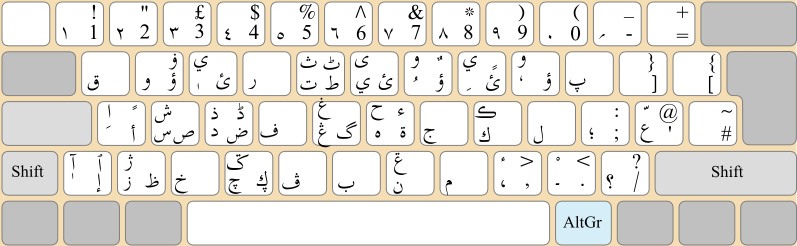
\includegraphics[keepaspectratio=true, scale=0.7]{./images/Swahili_keyboard.png}
 % Swahili_keyboard.png: 797x246 pixel, 90dpi, 22.50x6.94 cm, bb=0 0 638 197
 \caption{Keyboard layout for writing Swahili in Arabic script}
 \label{fig:kblayout}
\end{figure}

As can be seen from Figure \ref{fig:kblayout}, up to four glyphs may be accessed from one key.  To access the contents of each key, the \textbf{Shift} and \textbf{AltGr} keys are used in combination where appropriate, as shown in \Cref{fig:key}.

\begin{figure}[!ht]
 \centering
 \includegraphics[keepaspectratio=true, scale=1]{./images/key.png}
 % key.png: 562x100 pixel, 90dpi, 15.86x2.82 cm, bb=0 0 450 80
 \caption{Accessing the glyphs on the keys}
 \label{fig:key}
\end{figure}

\section{Governing principles for the layout}

The basic governing principle behind the keyboard layout is that the relevant Arabic glyph will usually be produced by pressing the same key that produces the Roman glyph.  It is thus very easy to use: just switch your keyboard to use Arabic script -- in KDE, \textbf{Ctrl+Alt+K} (see \Cref{s:kbactivate} for further information) -- and start typing almost as if the keyboard is being used to type Roman script.  Some examples are given in \Cref{tab:typeeg}.\footnote{For an explanation of the penultimate long vowels accessed by the Shift keys, see \Cref{ch:spelling}.}

\begin{table}[h!]
\centering
\begin{tabularx}{10cm}{rlll}
\textbf{Arabic} & \textbf{Keystrokes} & \textbf{Roman} & \textbf{English}\\
\hline\noalign{\smallskip}
\AS{مِيمِ} & m, i, Shift+i, m, i & mimi & I, me \\
\AS{سَاسَ} & s, a, Shift+a, s, a & sasa & now \\
\AS{لَكِينِ} & l, a, k, i, Shift+i, n, i & lakini & but \\
\AS{نِمٖفِيكَ} & n, i, m, e, f, i, Shift+i, k, a & nimefika & I have arrived \\
\end{tabularx}
\caption{Typing examples}
\label{tab:typeeg}
\end{table}

The other main principle behind the layout is the consistent placement of glyphs that are related by shape or sound in either script:
\begin{itemize}
\item The digraphs \textbf{dh gh th sh} are on the same keys as \textbf{d g t s}, and are accessed using the \textbf{Shift} key.
\item The pharyngeal consonants \AS{ص ض ط ظ} are on the same keys as \textbf{z t d s}, and are accessed using the \textbf{AltGr} key.
\item Similar Arabic glyph shapes are placed on the same key where possible -- for instance \AS{ي ى} are on the \textbf{y} key, and \AS{و ۏ} are on the \textbf{w} key.
\item Long and short vowels are located on the same key, with the long vowel accessed by \textbf{Shift}, so for instance the \textbf{u} key produces \AS{ُ } and \textbf{Shift+u} produces \AS{و}.
\item The vowel carriers \AS{أ إ ئ ؤ} are all accessed using the\textbf{AltGr} key.
\item The alveolar consonants \AS{ٹ ڈ} used in Mombasa Swahili are accessed using the \textbf{Shift+AltGr} keys.
\item The glyphs \AS{و ي} are repeated on \textbf{w y} for use when they represent semi-vowels.
\item The palatal digraph \textbf{ch} is accessed using the \textbf{c} key, and an alternate representation used by some writers, \AS{\char"063B}, is accessed using \textbf{Shift+c}.
\item The occasionally-used digraph \textbf{kh} is accessed using the \textbf{X} key.
\item Non-alphabetic characters from the UK keyboard are currently available via \textbf{AltGr} and \textbf{AltGr+Shift}, in case they might be of use.
\end{itemize}

Further information on the glyphs accessible from each key is available in the tables in \Cref{ch:spelling}.

\section{Changing the layout}
\label{s:changelayout}

The layout of the keyboard is specified in the file \textit{layout/tz}.  Once copied to the appropriate place (see \Cref{s:keyboard}), the layout is available for use.  The file (reproduced in \Cref{appE}) is a simple text file, and can be easily adapted to add new glyphs or change the position of existing glyphs.

Each line follows the pattern below:

\verb|key <AC03> { [Arabic_dal, Arabic_thal, Arabic_dad, Arabic_ddal] };|

The key number (in this case AC03, for the \textbf{D} key) is followed by a sequence of 4 glyph names (in this case representing \AS{ڈ ض ذ د}).  The sequence specifies the glyph that will be output when (respectively) the user presses \textbf{D}, \textbf{Shift+D}, \textbf{AltGr+D}, and \textbf{Shift+AltGr+D}.

Some lines have less than four entries.  For instance, the \textbf{P} key only has one entry (\AS{پ}):

\verb|key <AD10> { [Arabic_peh] };|

because that is the only glyph output by that key, and the \textbf{S} key only has three entries ( \AS{ص ش س}):

\verb|key <AC02> { [Arabic_seen, Arabic_sheen, Arabic_sad] }|

giving the glyphs that will be output by pressing \textbf{S}, \textbf{Shift+S} and \textbf{AltGr+S}.

If it is desired to block one of the slots, to enforce a particular keypress for a glyph, the entry \verb|NoSymbol| can be used.  Thus in the line for the \textbf{5} key:

\verb|key <AE05> { [Arabic_5, NoSymbol, KP_5, percent] };|

the output will be \AS{٥} for \textbf{5}, nothing for \textbf{Shift+5}, Western 5 for \textbf{AltGr+5} and a percent sign for \textbf{Shift+AltGr+5}.  Without the \verb|NoSymbol|, the output would be \AS{٥} for \textbf{5}, Western 5 for \textbf{Shift+5}, a percent sign for \textbf{AltGr+5} and nothing for \textbf{Shift+AltGr+5}.

Glyph names are available for some, but by no means all, of the possible glyphs.\footnote{\url{http://wiki.linuxquestions.org/wiki/List_of_Keysyms_Recognised_by_Xmodmap}}  Where no name is available, the Unicode codepoint can be used instead.  Thus, in the line for the \textbf{n} key:

\verb|key <AB06> { [Arabic_noon, U075D] };|

\AS{ن} will be output when the \textbf{N} key is pressed, and the glyph represented by Unicode 075D (\AS{ݝ}, \textit{ain} with two dots above) will be output when \textbf{Shift+N} is pressed.  It would be possible to use nothing but Unicode codepoints in the file, but using the glyph names makes it a bit easier to read.

From the above, it will be obvious that adjusting the location of a particular glyph merely consists of moving it to the desired slot on the desired key.  For example, if the user wanted \AS{ض} to appear when Shift+D is pressed, and \AS{ذ} when AltGr+D is pressed, all that needs to be done is to open the file:

\verb|sudo nano layout/tz|

and change the line:

\verb|key <AC03> { [Arabic_dal, Arabic_thal, Arabic_dad, Arabic_ddal] };|

to:

\verb|key <AC03> { [Arabic_dal, Arabic_dad, Arabic_thal, Arabic_ddal] };|

Then save the file by pressing \textbf{Ctrl+X}, \textbf{Y}, and \textbf{Return}.

Likewise, adding a new glyph to the keyboard is as simple as deciding which slot on which key it should occupy, and then inserting the Unicode codepoint (or the glyph name where one exists) at that slot.  For instance, if the user needs to access the glyph \textit{rreh} (\textit{ra} with \textit{tah} as a diacritic, Unicode 0691), and decides to put it on the \textbf{R} key so that it will be output when \textbf{AltGr+R} is pressed, all that needs to be done is to change the line:

\verb|key <AD04> { [Arabic_ra] };|

to:

\verb|key <AD04> { [Arabic_ra, NoSymbol, U0691] };|

(Remember that if \verb|NoSymbol| is omitted here, \textit{rreh} will appear when \textbf{Shift+R} is pressed.)

In either case, the new layout has to be activated.  So, after saving the file, copy it to the correct location:

\verb|sudo cp layout/tz /usr/share/X11/xkb/symbols/|

Delete the cache files relating to the old layout (new ones will be created when the new layout is activated):

\verb|sudo rm /var/lib/xkb/server-*|

Then remove the \textit{tz} keyboard layout using your desktop's language setup utility and re-add it.  For KDE, this simply means going to \textbf{K} \textrightarrow\ \textbf{Settings} \textrightarrow\ \textbf{System Settings} \textrightarrow\ \textbf{Input Devices} \textrightarrow\ \textbf{Keyboard} \textrightarrow\ \textit{Layouts} tab, unticking \textbf{Configure layouts}, clicking \textbf{Apply}, and then reticking \textbf{Configure layouts} and clicking \textbf{Apply} again.

The new layout should then be ready for use.
